\subsection{Descripci�n del algoritmo}
Este algoritmo parte de un camino inicial $C$ vac�o. 
Luego, toma el nodo inicial $v$, recorre las aristas adyacentes cuyos nodos incidentes no est�n 
marcados como visitados. Para cada arista, chequea que al agregarla siga teniendo una soluci�n factible. Si es as�, y el otro extremo 
$w$ de la arista no est� marcado como visitado, 
agrega la arista, se para en ese nodo, y chequea si es igual al nodo final. Si lo es, compara el camino obtenido con $C$,
y almacena
en $C$ el de menor peso respecto a W2. Luego marca como nodo inicial a $w$, marca como visitado a $v$ y repite recursivamente
el proceso. Esto es b�sicamente una resoluci�n con backtracking. 


\subsection{Complejidad}

\begin{algoritmo}{HallarCaminoMinimoAcotadoPorK}{grafo, verticeActual, verticeDestino, K, camino, caminoMinimo}
\;
  Visitar(verticeActual, grafo)	\tcc*{$O$(1)}\;
  
  \For(\tcc*[f]{$O$(|AristasIncidentesA(verticeActual, grafo)| * )}){\Forcond{e \asignar AristasIncidentesA(verticeActual, grafo)}}{
  
    vecino $\leftarrow$ ObtenerVerticeVecinoA(verticeActual, e) \tcc*{$O$(1)}\;
  
    \If(\tcc*[f]{$O$(1)}){PesoTotalEnW1(camino) + PesoW1(e) < K $\wedge$ $\neg$FueVisitado(vecino)}{
    
      \uIf(\tcc*[f]{$O$(1)}){vecino $\not=$ verticeDestino}{ \tcc*{$O$(1)}
	
	AgregarArista(e, camino)	\tcc*{$O$(1)}\; 
	HallarCaminoMinimoAcotadoPorK(grafo, vecino, verticeDestino, K, camino, caminoMinimo)	\;
	RemoverArista(e, camino)	\tcc*{$O$(1)}\;
             
      }\Else{
      
	AgregarArista(e, camino)	\tcc*{$O$(1)}\;
	caminoMinimo \asignar ObtenerElCaminoMinimoEntre(camino, caminoMinimo)	\tcc*{$O$(|camino|)}\;
	RemoverArista(e, camino)	\tcc*{$O$(1)}\;
      
      }
      
    }
    
  }
  
  Desvisitar(verticeActual, grafo)	\tcc*{$O$(1)}\;
\end{algoritmo}

Complejidad Total: Este algoritmo es recursivo. Para cada nodo recorre a lo sumo todas las aristas, pero podemos acotar esto sabiendo 
que si visitamos un nodo en la K-esima llamada, ya habremos 
marcado como visitados a k nodos antes, por lo que solo recorrer�a en el peor caso $n-k$ aristas, porque solo puede tener $n-1$ aristas
incidentes, y as� recursivamente, 
donde $n$ es la cantidad inicial de nodos. Luego la complejidad de este algoritmo es
$\Pi_{k=1}^{n} n-k $. Por lo tanto, la complejidad en el peor caso de este algoritmo es $(n-1)!$.

\subsection{Experimentaci�n}

Para la medici�n de tiempo de este algoritmo, creamos un generados de grafos aleatorio. El gr�fico 
que presentemos esta contantizado, es decir,
las mediciones fueron divididas por la complejidad que calculamos en el punto anterior. Ac� esperar�amos observar 
una constante pero 
dado que la complejidad de este algoritmo es factorial, las muestras que podemos son muy peque�as, por lo que el 
gr�fico no puede presentar las 
suficientes muestras para que la curvatura de la funci�n tienda a algo. Sin embargo, podemos ver que el gr�fico se 
mantiene cerca del eje x, lo que 
nos indica que claramente la complejidad esta acotada por la calculada.

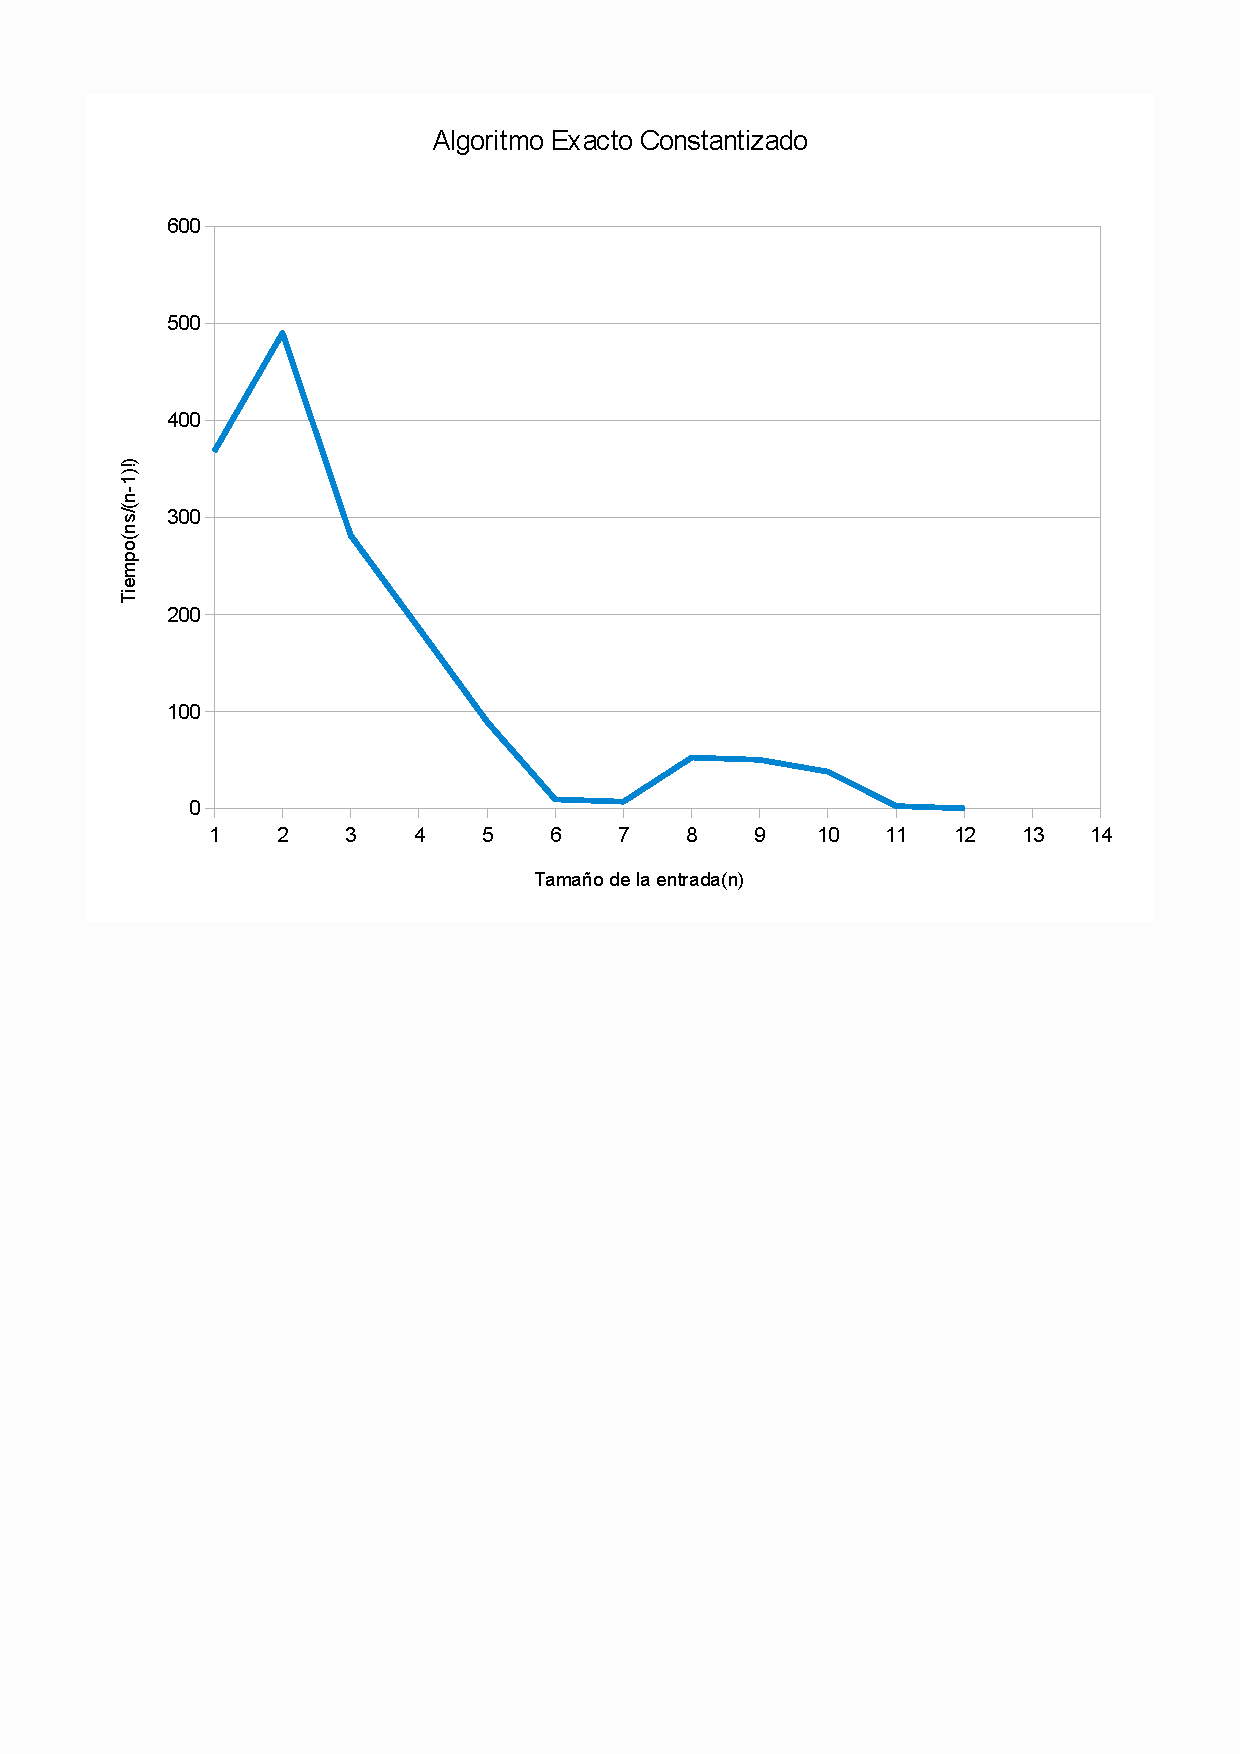
\includegraphics[width=1\textwidth]{exacto_grafico.pdf}[!]